\chapter{Inverse of Infinite Matrices}
This chapter delves into inverse matrices, with Section 1 concentrating on finite matrices and defining matrix inverses, accompanied by an illustrative example. In Section 2, the discussion extends to infinite matrices, introducing a corollary on the determinant relationship in matrix products. A proposition outlines conditions for expressing the inverse of a matrix as an infinite series, contingent upon the convergence of matrix rows and columns, along with the sub-multiplicative norm of the matrix difference being less than 1. A practical example involving finite matrices is provided for clarity.Here, we follow most of the definitions from the classical book  Richard E. Bellman~\cite{bellman1997introduction} and the article P.N. Shivakumar~\cite{infinite_PN_SHIVA_2009}.



\section{Inverse of a finite matrix}
Let $A$ be a square matrix. Then $A$ is \textbf{invertible} if there exits a matrix $B$ such that $AB = BA = I$. Then we call the matrix $B$, the \textbf{inverse} of $A$, and write $B = A^{-1}$.

For example, consider the following matrices $A$ and $B$. 
\[
    A = 
    \begin{bmatrix}
    1 & 0 & 0\\
    0 & 1 & 0\\
    0 & -4 & 1
\end{bmatrix}
~B =
\begin{bmatrix}
    1 & 0 & 0\\
    0 & 1 & 0\\
    0 & 4 & 1
\end{bmatrix}
\]

We find that
\[ 
    AB = 
    \begin{bmatrix}
    1 & 0 & 0\\
    0 & 1 & 0\\
    0 & -4 & 1
\end{bmatrix}
\begin{bmatrix}
    1 & 0 & 0\\
    0 & 1 & 0\\
    0 & 4 & 1
\end{bmatrix}
= I
\]

and
\[ 
    BA = 
    \begin{bmatrix}
    1 & 0 & 0\\
    0 & 1 & 0\\
    0 & 4 & 1
\end{bmatrix}
\begin{bmatrix}
    1 & 0 & 0\\
    0 & 1 & 0\\
    0 &-4 & 1
\end{bmatrix}
= I.
\]

Therefore, $A^{-1} = B$.   


\vspace{30pt}
\section{Inverse of an infinite matrix}

\begin{definition}
$A$ matrix $A \in M_{n}(K) $ (where $n \in \mathbb{N} \cup \{\infty\}$ , $K$ be a field) is \textbf{invertible} if and only if the map $f : K^{n} \to K^{n}$ defined by $f(x) = Ax$ is invertible, where elements of $K^{n}$ are considered as column vectors. 
\end{definition}

\begin{example}
Let \( K = \mathbb{R} \) (the field of real numbers) and consider the following matrix \( A \in M_2(\mathbb{R}) \)

\[ A = \begin{bmatrix} 2 & 1 \\ 1 & 3 \end{bmatrix} \]

Now, let's define the map \( f : \mathbb{R}^2 \to \mathbb{R}^2 \) by \( f(x) = Ax \), where \( x \) is a column vector in \( \mathbb{R}^2 \). The matrix-vector multiplication \( Ax \) corresponds to the standard matrix multiplication.

If \( x = \begin{bmatrix} x_1 \\ x_2 \end{bmatrix} \), then

\[ Ax = \begin{bmatrix} 2x_1 + x_2 \\ x_1 + 3x_2 \end{bmatrix} \]

Now, let's check if the map \( f \) is invertible. According to the theorem, the matrix \( A \) is invertible if and only if \( f \) is invertible.

To find the inverse of \( A \), you can use the formula for the inverse of a 2x2 matrix

\[ A^{-1} = \frac{1}{\text{det}(A)} \begin{bmatrix} 3 & -1 \\ -1 & 2 \end{bmatrix} \]

Here, \( \text{det}(A) \) is the determinant of \( A \), which is \( (2 \times 3) - (1 \times 1) = 5 \). Therefore,

\[ A^{-1} = \frac{1}{5} \begin{bmatrix} 3 & -1 \\ -1 & 2 \end{bmatrix} \]

Now, \( f \) has an inverse, and you can verify that \( f^{-1}(y) = A^{-1}y \). This means that \( f \) is an invertible map.

So, the matrix \( A = \begin{bmatrix} 2 & 1 \\ 1 & 3 \end{bmatrix} \) is invertible, and the map \( f(x) = Ax \) is invertible as well.


\end{example}

%For infinite matrices, we put $\infty$-tuple in proof in the form $(k_1, k_2, k_3, \ldots)$. And put $1 \leq j_1, j_2, j_3, \ldots < n = \infty$.\cite{amgopaper}


%\begin{corollary}
%    f $m = n$ ($m, n \in \mathbb{N} \cup \{\infty\}$), then
%\[\det(AB) = \det(A) \det(B).\]
%\end{corollary}

The following proposition gives us a way to compute the inverse of an infinite matrix.

\begin{proposition}\label{inverse_geometric} \cite{amgopaper} Let $A$ be a matrix in which every row and column forms a convergent series such that $\|I - A\| < 1$, where $\|\cdot\|$ is a submultiplicative norm. Then
\[ A^{-1} = I + (I -A ) + (I - A)^2 + \cdots.\]
\end{proposition}

\begin{proof}
 We see that $I + (I -A ) + (I - A)^2 + \cdots$ is a geometric series with $I-A$ as the ratio of the consecutive terms of the series. Since $\|I - A\| < 1$, we have the sum of the series as follows:
     \[I + (I -A ) + (I - A)^2 + \cdots = \frac{I}{I-(I-A)} = \frac{I}{A} = A^{-1}.\]
\end{proof}

We illustrate the above result in the following two examples in the case of finite matrices with submultiplicative norms less than 1.

\begin{example}
 Let
\[ A = 
\begin{bmatrix}
    0.6015 & 0.6618 & 0.1938 \\
   -0.4642 & 1.0997 & -0.6004 \\
   -0.2306 & -0.1662 & 1.5319
\end{bmatrix}.
\]
\newline
% By using Source Code \ref{sourcecode-matrix-inverse} we know that the submultiplicative norm of $A$ is $0.8804410$. Therefore, $A$ is invertible. 
We see that the submultiplicative norm of $A$ is $0.8804410$. Thus, $A$ is invertible. 
\newline

We use the MATLAB code Source Code~\ref{sourcecode-matrix-inverse} (Algorithm~\ref{alg:inverse_matrices}) to compute the terms $(I-A)^{n}$ of the following series $A^{-1} = I + (I -A ) + (I - A)^2 + \cdots$ up to $42$ terms terms. Some of the terms are given as follows:\newline   
%%%To converge upto 6 decimal places it takes around these number of steps 42 %%%%
\[
I - A =
\begin{bmatrix}
    0.3985 & -0.6618 & -0.1938 \\
    0.4642 & -0.0997 & 0.6004 \\
    0.2306 & 0.1662 & -0.5319
\end{bmatrix}
\]
\newline
\[
(I - A)^2 =
\begin{bmatrix}
   -0.1931 & -0.2300 & -0.3715 \\
    0.2772 & -0.1975 & -0.4692 \\
    0.0464 & -0.2576 & 0.3380
\end{bmatrix}
\]
\newline
\[
(I - A)^3 =
\begin{bmatrix}
   -0.2693 & 0.0889 & 0.0969 \\
   -0.0894 & -0.2417 & 0.0773 \\
   -0.0231 & 0.0512 & -0.3434
\end{bmatrix}
\]
\newline
\[
(I - A)^4 =
\begin{bmatrix}
   -0.0437 & 0.1855 & 0.0540 \\
   -0.1300 & 0.0961 & -0.1689 \\
   -0.0647 & -0.0469 & 0.2179
\end{bmatrix}
\]
\newline
\[
(I - A)^5 =
\begin{bmatrix}
    0.0811 & 0.0194 & 0.0911 \\
   -0.0461 & 0.0484 & 0.1727 \\
    0.0027 & 0.0837 & -0.1315
\end{bmatrix}
\]
\newline

Finally, we have

\[ A^{-1} =
\begin{bmatrix}
    1.0034 & -0.6622 & -0.3864 \\
    0.5379 & 0.6116 & 0.1717 \\
    0.2094 & -0.0333 & 0.6132
\end{bmatrix}.
\]
\newline
\newline
\newline

The graphical representation in Figure~\ref{graph-inverse-01} illustrates the diminishing error in the computation of the inverse of a finite matrix with an increasing number of iterations. Specifically, the analysis focuses on 42 iterations, utilizing a logarithmic scale to quantify the error. The graphical depiction strongly implies that the iterative process for determining the inverse matrix exhibits rapid and precise convergence, attesting to its efficiency and accuracy.

\begin{center}
    \begin{figure}[h]
        \centering
        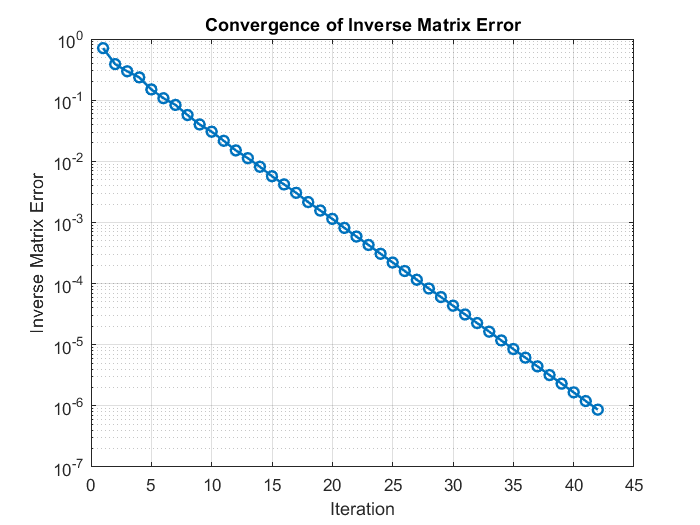
\includegraphics[width=0.7\linewidth]{Figures/for_the_first_one.png}
        \caption{Error plot during iterative inverse computation (Case 1)}
        \label{graph-inverse-01}
    \end{figure}
\end{center}

\end{example}
\newpage
\begin{example}
\label{inverse}
Let
\[
B = 
\begin{bmatrix}
    1.2000 & -0.0200 & -0.1200 & -0.0600 & -0.0800 & -0.0030 & -0.0050 \\
   -0.0800 & 0.9997 & -0.0030 & -0.0400 & -0.0200 & -0.0070 & -0.0060 \\
   -0.0100 & -0.0100 & 0.9997 & -0.0060 & -0.0070 & -0.0040 & -0.0006 \\
   -0.0300 & -0.0100 & -0.0200 & 0.9994 & -0.0200 & -0.0500 & -0.0700 \\
   -0.0300 & -0.2141 & -0.0007 & -0.0942 & 0.9999 & -0.0009 & -0.0001 \\
   -0.0800 & -0.0120 & -0.0004 & -0.0009 & -0.9890 & 0.9994 & -0.0005 \\
   -0.0300 & -0.0010 & -0.0050 & -0.0020 & 0 & -0.3000 & 0.9998
\end{bmatrix}.
\]

We see that the submultiplicative norm of $B$ is $0.995135$. Therefore, $B$ is invertible. 

We use the MATLAB code Source Code~\ref{sourcecode-matrix-inverse} (Algorithm~\ref{alg:inverse_matrices}) to compute the terms $(I-B)^{n}$ of the series $B^{-1} = I + (I -B ) + (I - B)^2 + \cdots$ up to $29$ terms. We find
% Some of the terrm %%%%%%%%%%%%%%
\[
(I-B) = \begin{bmatrix}
   -0.2000 & 0.0200 & 0.1200 & 0.0600 & 0.0800 & 0.0030 & 0.0050 \\
    0.0800 & 0.0003 & 0.0030 & 0.0400 & 0.0200 & 0.0070 & 0.0060 \\
    0.0100 & 0.0100 & 0.0003 & 0.0060 & 0.0070 & 0.0040 & 0.0006 \\
    0.0300 & 0.0100 & 0.0200 & 0.0006 & 0.0200 & 0.0500 & 0.0700 \\
    0.0300 & 0.2141 & 0.0007 & 0.0942 & 0.0001 & 0.0009 & 0.0001 \\
    0.0800 & 0.0120 & 0.0004 & 0.0009 & 0.9890 & 0.0006 & 0.0005 \\
    0.0300 & 0.0010 & 0.0050 & 0.0020 & 0 & 0.3000 & 0.0002
\end{bmatrix}
\]

\[
(I-B)^2 = \begin{bmatrix}
   -0.0134 & 0.0064 & 0.0104 & 0.0068 & 0.0142 & 0.0041 & 0.0032 \\
    0.0005 & 0.0018 & 0.0014 & 0.0017 & 0.0051 & 0.0006 & 0.0005 \\
    0.0036 & 0.0116 & 0.0004 & 0.0053 & 0.0215 & 0.0004 & 0.0004 \\
   -0.0013 & 0.0026 & 0.0019 & 0.0019 & 0.0077 & 0.0030 & 0.0008 \\
    0.0175 & 0.0030 & 0.0044 & 0.0102 & 0.0089 & 0.0067 & 0.0083 \\
    0.0058 & 0.0645 & 0.0025 & 0.0295 & 0.0021 & 0.0006 & 0.0003 \\
    0.0182 & 0.0043 & 0.0038 & 0.0021 & 0.2992 & 0.0005 & 0.0004
\end{bmatrix}
\]

\[
(I-B)^3 = \begin{bmatrix}
   -0.0084 & -0.0015 & 0.0057 & 0.0023 & 0.0084 & 0.0010 & 0.0001 \\
    0.0017 & 0.0030 & -0.0014 & 0.0009 & 0.0033 & 0.0014 & 0.0005 \\
    0.0036 & 0.0116 & 0.0004 & 0.0053 & 0.0215 & 0.0004 & 0.0004 \\
   -0.0013 & 0.0026 & 0.0019 & 0.0019 & 0.0077 & 0.0030 & 0.0008 \\
    0.0175 & 0.0030 & 0.0044 & 0.0102 & 0.0089 & 0.0067 & 0.0083 \\
    0.0058 & 0.0645 & 0.0025 & 0.0295 & 0.0021 & 0.0006 & 0.0003 \\
    0.0050 & 0.0009 & 0.0015 & 0.0032 & 0.0030 & 0.0020 & 0.0025
\end{bmatrix}
\]

\[
(I-B)^4 = \begin{bmatrix}
    0.0020 & 0.0017 & -0.0010 & 0.0003 & 0.0004 & 0.0001 & 0.0001 \\
   -0.0004 & 0.0008 & 0.0006 & 0.0007 & 0.0018 & 0.0002 & 0.0001 \\
    0.0000 & 0.0002 & 0.0001 & 0.0001 & 0.0003 & 0.0001 & 0.0000 \\
    0.0011 & 0.0047 & 0.0006 & 0.0027 & 0.0011 & 0.0005 & 0.0005 \\
    0.0010 & 0.0017 & -0.0001 & 0.0008 & 0.0030 & 0.0004 & 0.0001 \\
   -0.0019 & 0.0025 & 0.0024 & 0.0021 & 0.0083 & 0.0031 & 0.0008 \\
    0.0050 & 0.0009 & 0.0015 & 0.0032 & 0.0030 & 0.0020 & 0.0025
\end{bmatrix}
\]



%%%%%%%% Here write replace the value of a as (I - A) , (I-A)^2 ... and define I
\[
B^{-1} =
\begin{bmatrix}
    0.8408 & 0.0354 & 0.1023 & 0.0600 & 0.0787 & 0.0089 & 0.0087 \\
    0.0708 & 1.0110 & 0.0126 & 0.0485 & 0.0396 & 0.0128 & 0.0098 \\
    0.0101 & 0.0132 & 1.0017 & 0.0084 & 0.0132 & 0.0050 & 0.0013 \\
    0.0367 & 0.0326 & 0.0252 & 1.0135 & 0.0959 & 0.0727 & 0.0714 \\
    0.0440 & 0.2208 & 0.0089 & 0.1078 & 1.0209 & 0.0108 & 0.0092 \\
    0.1117 & 0.2336 & 0.0175 & 0.1130 & 1.0173 & 1.0124 & 0.0105 \\
    0.0589 & 0.0723 & 0.0134 & 0.0378 & 0.3079 & 0.3042 & 1.0038
\end{bmatrix}
\]

The graph in Figure~\ref{graph-inverse-02} visually represents the decreasing error in computing the inverse of a finite matrix as the number of iterations increases, with a specific focus on 29 iterations. Employing a logarithmic scale to measure the error, the illustration strongly suggests that the iterative process for determining the inverse matrix converges swiftly and accurately, highlighting its efficiency and precision.

\begin{center}
    \begin{figure}[h]
        \centering
        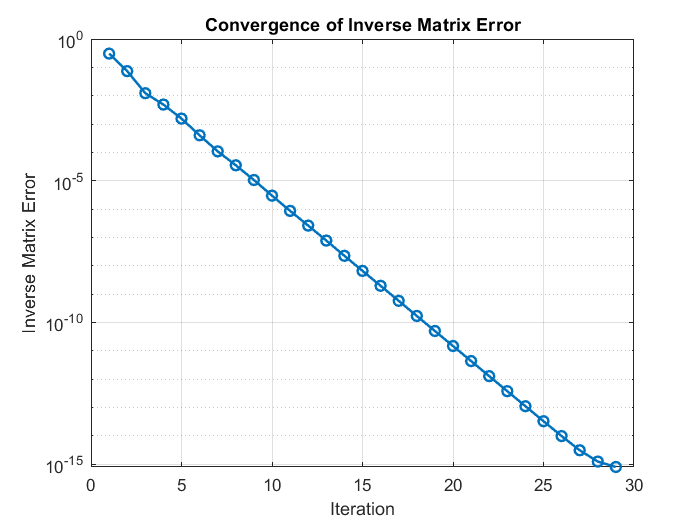
\includegraphics[width=0.8\linewidth]{Figures/inverse_erorr_fig.png}
        \caption{Error plot during iterative inverse computation (Case 2)}
        \label{graph-inverse-02}
    \end{figure}
\end{center}


We observe that
\[B B^{-1}=
\begin{bmatrix}
    1.0000 & -0.0000 & -0.0000 & -0.0000 & -0.0000 & -0.0000 & -0.0000 \\
   -0.0000 & 1.0000 & -0.0000 & -0.0000 & -0.0000 & -0.0000 & -0.0000 \\
   -0.0000 & -0.0000 & 1.0000 & -0.0000 & -0.0000 & -0.0000 & -0.0000 \\
   -0.0000 & -0.0000 & -0.0000 & 1.0000 & -0.0000 & -0.0000 & -0.0000 \\
   -0.0000 & -0.0000 & -0.0000 & -0.0000 & 1.0000 & -0.0000 & -0.0000 \\
   -0.0000 & -0.0000 & -0.0000 & -0.0000 & -0.0000 & 1.0000 & -0.0000 \\
   -0.0000 & -0.0000 & -0.0000 & -0.0000 & -0.0000 & -0.0000 & 1.0000 \\
\end{bmatrix}.
\]
\end{example}

\bigskip






\section{Applications of matrix inverse}

We can represent any infinite system of linear equations by \(BX = C\), where \(B\) is the coefficient matrix, \(X\) is the column vector of variables, and \(C\) is the right-hand side vector of the constants. If \(B\) is an infinite square matrix and has its inverse then we can apply the matrix inverse method to solve an infinite system of linear equations represented by \(BX = C\). This method is illustrated in the following example in the case of a finite system of linear equations such that the coefficient matrix \(B\) satisfies the condition of sub-multiplicative norm.

\begin{example}
Consider the system of linear equations that takes the following matrix form.
\[\small
\begin{bmatrix}
  1.2 & -0.02 & -0.12 & -0.06 & -0.08 & -0.003 & -0.005\\
 -0.08 & 0.9997 & -0.003 & -0.040 & -0.02 & -0.007 & -0.006 \\
 -0.01 & -0.01 & 0.9997 & -0.006 & -0.007 & -0.004 & -0.0006 \\
 -0.03 & -0.01 & -0.02 & 0.9994 & -0.02 & -0.05 & -0.07 \\
 -0.03 & -0.2141 & -0.0007 & -0.0942 & 0.9999 & -0.0009 & -0.0001 \\
 -0.08 & -0.012 & -0.0004 & -0.0009 & -0.989 & 0.9994 & -0.0005 \\
  -0.03 & -0.001 & -0.0050 & -0.0020 & 0 & -0.3000 & 0.9998
\end{bmatrix}
\begin{bmatrix}
    x_1 \\
    x_2 \\
    x_3 \\
    x_4 \\
    x_5 \\
    x_6 \\
    x_7
\end{bmatrix}
=
\begin{bmatrix}
    0.1 \\
    0.2 \\
    0.3 \\
    0.4 \\
    0.5 \\
    0.6 \\
    0.7
\end{bmatrix}
\]

Now we solve this system of linear equations with the help of the inverse matrix as follows:

\[\small
\begin{bmatrix}
    x_1 \\
    x_2 \\
    x_3 \\
    x_4 \\
    x_5 \\
    x_6 \\
    x_7
\end{bmatrix}
=
\begin{bmatrix}
  1.2 & -0.02 & -0.12 & -0.06 & -0.08 & -0.003 & -0.005\\
 -0.08 & 0.9997 & -0.003 & -0.040 & -0.02 & -0.007 & -0.006 \\
 -0.01 & -0.01 & 0.9997 & -0.006 & -0.007 & -0.004 & -0.0006 \\
 -0.03 & -0.01 & -0.02 & 0.9994 & -0.02 & -0.05 & -0.07 \\
 -0.03 & -0.2141 & -0.0007 & -0.0942 & 0.9999 & -0.0009 & -0.0001 \\
 -0.08 & -0.012 & -0.0004 & -0.0009 & -0.989 & 0.9994 & -0.0005 \\
  -0.03 & -0.001 & -0.0050 & -0.0020 & 0 & -0.3000 & 0.9998
\end{bmatrix}^{-1}
\begin{bmatrix}
    0.1 \\
    0.2 \\
    0.3 \\
    0.4 \\
    0.5 \\
    0.6 \\
    0.7
\end{bmatrix}
\]

From Example \ref{inverse}, we can demonstrate that

\[
B^{-1} =
\begin{bmatrix}
    0.8408 & 0.0354 & 0.1023 & 0.0600 & 0.0787 & 0.0089 & 0.0087 \\
    0.0708 & 1.0110 & 0.0126 & 0.0485 & 0.0396 & 0.0128 & 0.0098 \\
    0.0101 & 0.0132 & 1.0017 & 0.0084 & 0.0132 & 0.0050 & 0.0013 \\
    0.0367 & 0.0326 & 0.0252 & 1.0135 & 0.0959 & 0.0727 & 0.0714 \\
    0.0440 & 0.2208 & 0.0089 & 0.1078 & 1.0209 & 0.0108 & 0.0092 \\
    0.1117 & 0.2336 & 0.0175 & 0.1130 & 1.0173 & 1.0124 & 0.0105 \\
    0.0589 & 0.0723 & 0.0134 & 0.0378 & 0.3079 & 0.3042 & 1.0038
\end{bmatrix}.
\]

Then
\[\small
\begin{bmatrix}
    x_1 \\
    x_2 \\
    x_3 \\
    x_4 \\
    x_5 \\
    x_6 \\
    x_7
\end{bmatrix}
=
\begin{bmatrix}
    0.8408 & 0.0354 & 0.1023 & 0.06 & 0.0787 & 0.0089 & 0.0087 \\
    0.0708 & 1.011 & 0.0126 & 0.0485 & 0.0396 & 0.0128 & 0.0098 \\
    0.0101 & 0.0132 & 1.0017 & 0.0084 & 0.0132 & 0.005 & 0.0013 \\
    0.0367 & 0.0326 & 0.0252 & 1.0135 & 0.0959 & 0.0727 & 0.0714 \\
    0.044 & 0.2208 & 0.0089 & 0.1078 & 1.0209 & 0.0108 & 0.0092 \\
    0.1117 & 0.2336 & 0.0175 & 0.113 & 1.0173 & 1.0124 & 0.0105 \\
    0.0589 & 0.0723 & 0.0134 & 0.0378 & 0.3079 & 0.3042 & 1.0038
\end{bmatrix}
\begin{bmatrix}
    0.1 \\
    0.2 \\
    0.3 \\
    0.4 \\
    0.5 \\
    0.6 \\
    0.7
\end{bmatrix}.
\]
By matrix multiplication, we have
\[ 
\begin{bmatrix}
    x_1 \\
    x_2 \\
    x_3 \\
    x_4 \\
    x_5 \\
    x_6 \\
    x_7
\end{bmatrix}
=
\begin{bmatrix}
    0.1966 \\
    0.2668 \\
    0.3180 \\
    0.5647 \\
    0.6177 \\
    1.2318 \\
    1.0786
\end{bmatrix}.
\]

 So we find the unknown variables
 $x_1 = 0.1966, x_2 = 0.2668, x_3 = 0.3180, x_4 = 0.5647, x_5 = 0.6177, x_6 = 1.2318$, and $x_7 = 1.0786 .$

\end{example}